\section{トランジット現象 \label{ss:transit}}

\begin{figure}[]
 \begin{center}
	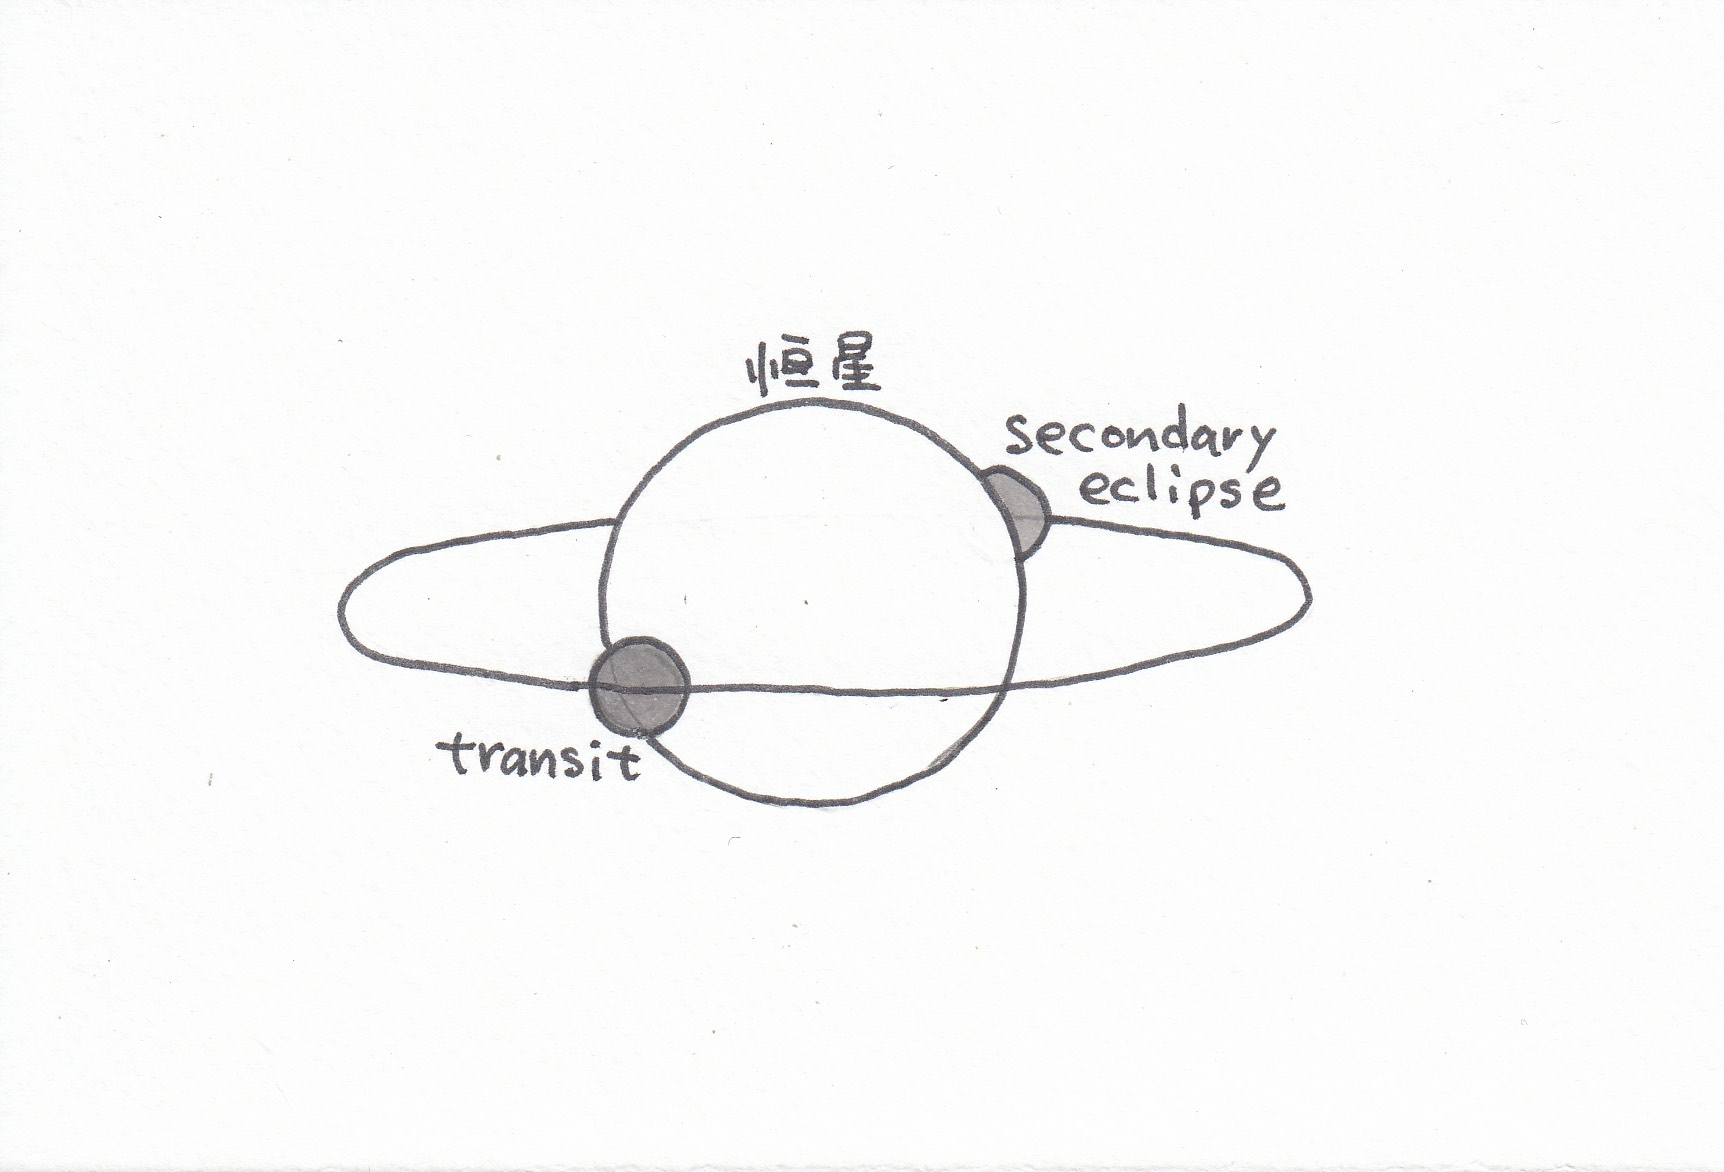
\includegraphics[width=\linewidth]{fig/transit.jpg}
	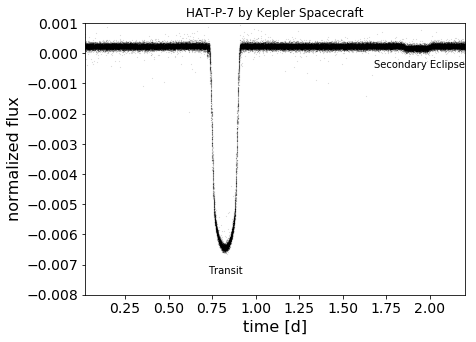
\includegraphics[width=\linewidth]{fig/Hatp7.png}
 \end{center}
 \caption{トランジット系の概念図(上)とホットジュピターHAT-P-7bによるトランジット減光曲線の例(下)。\label{fig:hatp7b}}
\end{figure} 

主星フラックスの変動にも惑星によるシグナルが含まれる。最も分かりやすいのは主星の前面を惑星が通過する時にできる陰によるフラックス減少である{\bf トランジット減光}\index{とらんじっとげんこう@トランジット減光}である(図\ref{fig:hatp7b})。トランジット系は逆に惑星が主星の後ろに隠れることによる減光も観測されている。後者は二次食\index{にじしょく@二次食}(secondary eclipse)\index{secondary eclipse@secondary eclipse}とか単にocclutation\index{occlutation@occlutation}と呼ばれている。

惑星がトランジットする確率は、円軌道かつ$R_p \ll R_\star$を仮定すると、図\ref{fig:transitprob}で示された領域であるから
\begin{align}
p_\mathrm{tra} = \sin{(R_\star/a)} \sim \frac{R_\star}{a} = 0.005 \left(\frac{R_\star}{R_\odot}\right) \left(\frac{a}{1 \mathrm{\, au}}\right)^{-1}
\label{eq:tranp}
\end{align}
となり、G型星まわりのハビタブル惑星だと0.5 \%である。


\begin{figure}[!hbt]
 \begin{center}
	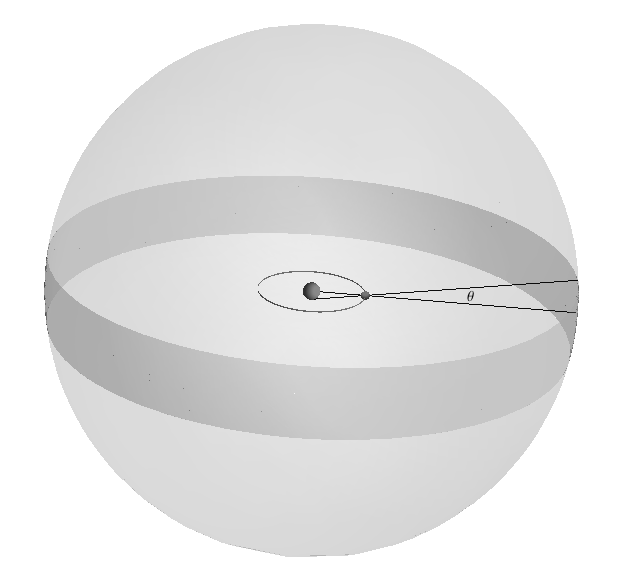
\includegraphics[width=\linewidth]{fig/transit_prob_bw.png}
\end{center}
	\caption{トランジットして見える立体角方向(帯部分)。中に恒星と惑星軌道が描かれている。外側の球の半径は、観測者から惑星系までの距離$d$であるので、$a \ll d$と見なせる。するとランダムな視線方向で帯領域をとる確率は$4 \pi \sin{\theta}/ (4 \pi) \approx R_\star/a$となる。\label{fig:transitprob}}
\end{figure} 

\subsection*{トランジットライトカーブ}

\begin{figure}[htb]
\begin{center}
	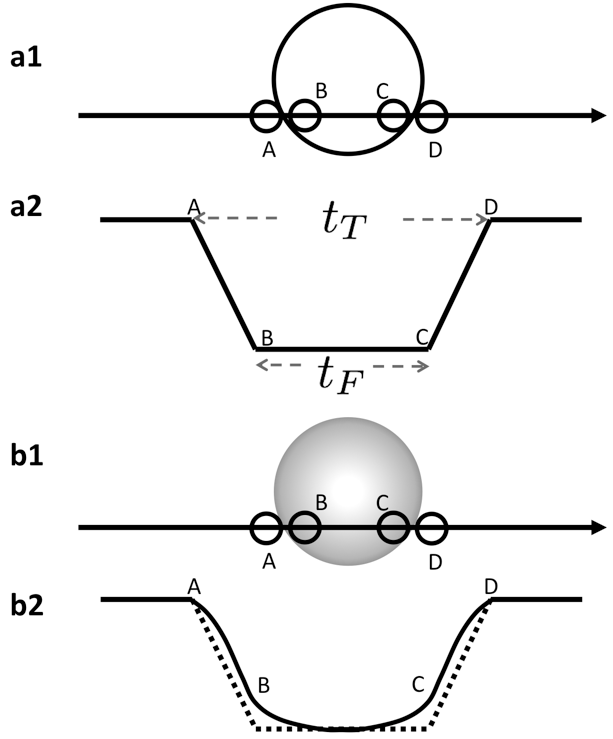
\includegraphics[width=\linewidth]{fig/transitmodel.png}
	\caption{トランジットライトカーブの幾何。aは恒星が一様に光っている場合のライトカーブ。実際は恒星は淵側が暗い(周辺減光)ためにbのようなライトカーブとなる。}
	\label{fig:transitmodel}
\end{center}
\end{figure} 

さてトランジットのライトカーブから、系外惑星系のどういった物理量が分かるのだろうか?まず複数回のトランジットが観測されれば、
\begin{itemize}
\item 公転周期$P$
\end{itemize}
を知ることができる。また、トランジット深さは、
\begin{itemize}
\item 惑星半径と恒星半径の比$k \equiv R_p/R_\star$
\end{itemize}
の二乗となるので、この$k$を知ることができる。トランジットの継続時間から
\begin{itemize}
\item 惑星の通過時間(duration) $T_\mathrm{tot}$
\end{itemize}
を知ることができる。さらに細かく見ると、もし恒星が一様に光っているという近似の元では、図\ref{fig:transitmodel}aに示されるように、ingress・egress時もわかる。つまり惑星が恒星に入るとき出る時に、惑星が恒星に入り始めてから、完全に出るまでの時間$t_T$と、惑星が完全に恒星の全面に入っている期間、$t_F$が測定できるというように言い換えることもできよう。恒星は、実際は周辺減光(Limb darkening)をしており、実際のライトカーブは図\ref{fig:transitmodel}bのようになる。そこで通常、周辺減光のモデル化を行うことで$t_T$と$t_F$も求めることができる。周辺減光のモデルとしては以下のquadratic limb-darkening law
\begin{align}
I(\mu) = I(\mu=1) [ 1 - u_1 (1 - \mu) - u_2 (1 -\mu)^2] 
\end{align}
がよく用いられる。ここに$\mu = \cos{\psi}$であり$\psi$は光球面の法線ベクトルと視線ベクトルのなす角度である。つまり中心で$\mu=1$、ディスク境界で$\mu=0$となる。上記モデルは円盤で積分すると$\pi R_\star^2 (1 - u_1/3 - u_2/6) I(\mu=1)$になることに注意。今、$k$がわかっているので、$t_T$, $t_F$から幾何学的に
\begin{itemize}
\item 衝突径数(impact parameter): $b = \frac{a}{R_\star} \cos{i} $
\end{itemize}
も知ることができる。恒星スペクトルのモデルや後述する恒星密度$\rho_\star$の情報を用いて$R_\star$と$M_\star$が推定できれば、周期$P$がわかっているとケプラー第3法則から$a$を推定することができる。これにより軌道傾斜角$i$を決定することができる。もし視線速度の測定されているトランジット系が存在すれば、軌道傾斜角$i$がわかっているので惑星質量$M_p$が求まるので、惑星の平均密度
\begin{align}
\rho_p \equiv \frac{3 M_p}{4 \pi R_p^3}
\end{align}
が推定できるということである。これにより系外惑星の大まかな分類が可能になった。

円軌道の場合、通過時間は$T_\mathrm{tot} = 2 \sqrt{1-b^2} R_\star/v$である。ここに$v$は惑星の通過速度である。
惑星の質量を無視したケプラー第三法則
\begin{align}
 P^2 = \frac{4 \pi^2}{G M_\star} a^3 
\end{align}
を$v=2 \pi a/P$であることに注意して変形すると
\begin{align}
v^3=2 \pi G M_\star/P 
\end{align}
となるので、$T_\mathrm{tot}^3 \propto  P/\rho_\star $となり、周期・衝突径数がわかっていると、通過時間からは恒星密度$\rho_\star$がわかることになる。逆にだいたいの通過時間を知っておくため $b=0$のときを書いてみよう。この場合、
\begin{align}
T_\mathrm{tot}  &= \left( \frac{3  P}{\pi^2 G \rho_\star} \right)^{1/3} \\
&= 2.6 \mathrm{h} \left(\frac{P}{3 \mathrm{day}}\right)^{1/3} \left(\frac{\rho_\star}{\rho_\odot}\right)^{-1/3} \\
&= 30  \mathrm{h} \left(\frac{P}{12 \mathrm{yr}}\right)^{1/3} \left(\frac{\rho_\star}{\rho_\odot}\right)^{-1/3} 
\end{align}
となる。二行目はホット・ジュピターの典型値で三番目は木星の場合を仮定している。このように周期が数年以上になっていくと、通過時間が一日を超えるようになってくる。また、巨星の場合は、恒星密度が桁で小さくなるので通過時間がやはり長くなる。

\begin{itembox}{{\it column} -- 周期とライトカーブ形状 $\,^\dagger$}
%\tiny
\footnotesize
円軌道を仮定すると幾何的考察からから、
\begin{align}
\label{eq:totald}
\sin{ \left( \frac{\pi t_T}{P} \right)}  = \frac{R_*}{a} \sqrt{\frac{(1+k)^2 - b^2}{\sin^2{i}}}, \\
\label{eq:totalf}
\sin{ \left( \frac{\pi t_F}{P} \right)}  = \frac{R_*}{a} \sqrt{\frac{(1-k)^2 - b^2}{\sin^2{i}}},
\end{align}
が得られる。ここで、$\sin{(\pi t_T/P)} \sim \pi t_T/P$、$\sin{(\pi t_F/P)} \sim \pi t_F/P$と近似すれば、
\begin{align}
\label{eq:ra}
\frac{R_\star}{a} = \frac{\pi}{2 \sqrt{k}} \frac{\sqrt{t_T^2 - t_F^2}}{P} \sin{i}.
\end{align}
が得られる。さらに惑星の質量を無視したケプラー第三法則
\begin{align}
 P^2 = \frac{4 \pi^2}{G M_\star} a^3 
\end{align}
を用い$\sin{i} \sim 1$とすると、
\begin{align}
\label{eq:pk}
P &= \frac{\pi G}{32} \frac{M_\star}{R_\star^3} \left( \frac{t_T^2 -t_F^2}{k} \right)^{\frac{3}{2}} \\
 &= \frac{\pi^2 G}{24} \rho_\star \left( \frac{t_T^2 -t_F^2}{k} \right)^{\frac{3}{2}} 
\end{align}
が得られる。最後の式で未知の量は、恒星の平均密度$\rho_\star$だけであり、トランジットライトカーブ解析から恒星の平均密度という物理量が分かることが示される。
\end{itembox}

\section{透過光分光スペクトル}

透過光分光はトランジット深さを波長方向に展開して測定する。波長依存性を含めたトランジット深さは
\begin{align}
\delta (\lambda) = \left( \frac{R_p(\lambda)}{R_\star} \right)^2
\end{align}
のように表される。ここでは恒星半径の波長依存性は無視している。ここに$R_p(\lambda)$は、光が透過しなくなる大気の高さに対応する半径となる。この高さは大気中の原子・分子吸収や散乱もしくは固体表面で決まる。図\ref{fig:transmission}に固体表面を持つ惑星に吸収のある分子を持つ大気がある場合の透過光分光の例を示す。分子吸収のない波長では、固体表面が$R_p$となる一方、吸収がある波長では大気中の光学的深さが1になる付近が$R_p$となるため、トランジット深さが少し深くなる。この違いを捉えることで大気中の分子を検出できる。この例では、分子吸収以外の波長の連続成分が固体表面で決まるとしたが、他の場合として、連続吸収やレイリー散乱、雲による散乱、強い吸収線のウイング、弱い多数の吸収線の集合であるpseudo continuumなどもありうる。

\begin{figure}[htb]
\begin{center}
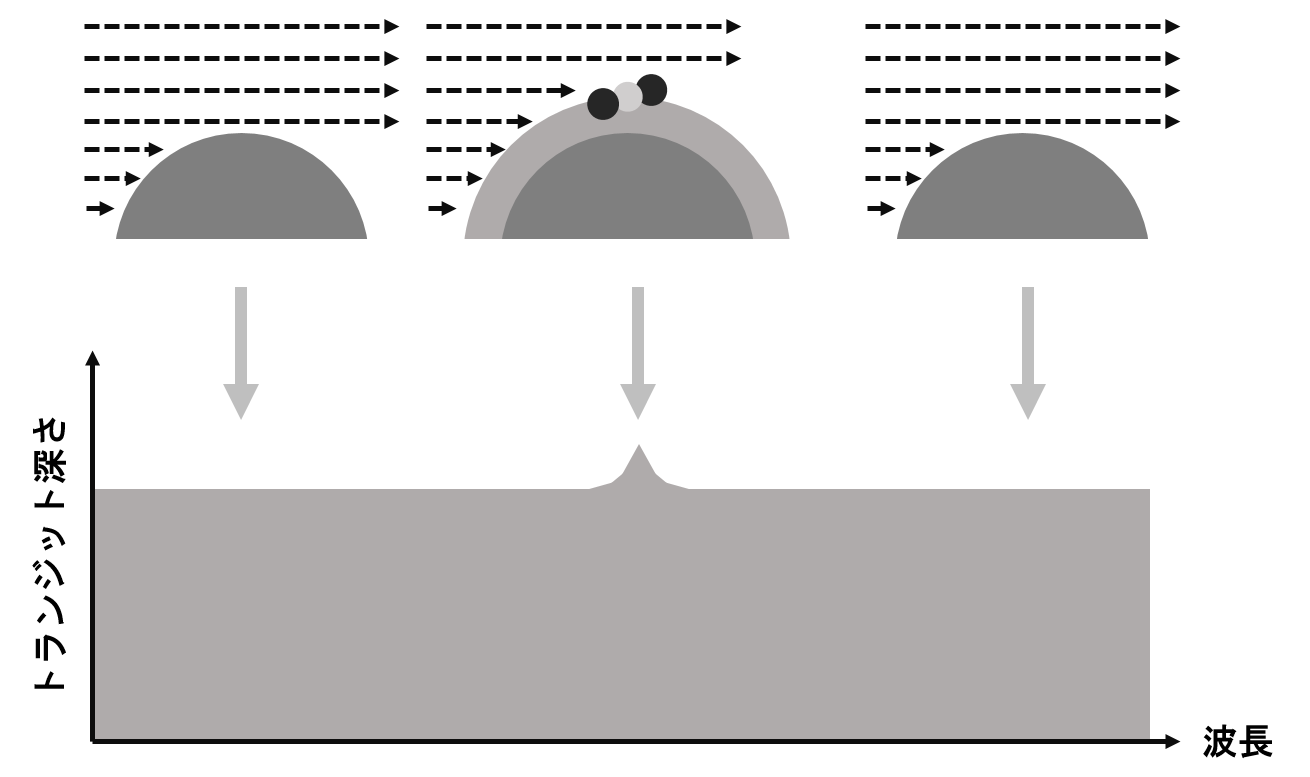
\includegraphics[width=\linewidth]{fig/transmission.png}
\caption{透過光分光の仕組み。\label{fig:transmission}}
\end{center}
\end{figure}

